% Options for packages loaded elsewhere
\PassOptionsToPackage{unicode}{hyperref}
\PassOptionsToPackage{hyphens}{url}
\PassOptionsToPackage{dvipsnames,svgnames,x11names}{xcolor}
%
\documentclass[
  letterpaper,
  DIV=11,
  numbers=noendperiod]{scrartcl}

\usepackage{amsmath,amssymb}
\usepackage{iftex}
\ifPDFTeX
  \usepackage[T1]{fontenc}
  \usepackage[utf8]{inputenc}
  \usepackage{textcomp} % provide euro and other symbols
\else % if luatex or xetex
  \usepackage{unicode-math}
  \defaultfontfeatures{Scale=MatchLowercase}
  \defaultfontfeatures[\rmfamily]{Ligatures=TeX,Scale=1}
\fi
\usepackage{lmodern}
\ifPDFTeX\else  
    % xetex/luatex font selection
\fi
% Use upquote if available, for straight quotes in verbatim environments
\IfFileExists{upquote.sty}{\usepackage{upquote}}{}
\IfFileExists{microtype.sty}{% use microtype if available
  \usepackage[]{microtype}
  \UseMicrotypeSet[protrusion]{basicmath} % disable protrusion for tt fonts
}{}
\makeatletter
\@ifundefined{KOMAClassName}{% if non-KOMA class
  \IfFileExists{parskip.sty}{%
    \usepackage{parskip}
  }{% else
    \setlength{\parindent}{0pt}
    \setlength{\parskip}{6pt plus 2pt minus 1pt}}
}{% if KOMA class
  \KOMAoptions{parskip=half}}
\makeatother
\usepackage{xcolor}
\setlength{\emergencystretch}{3em} % prevent overfull lines
\setcounter{secnumdepth}{5}
% Make \paragraph and \subparagraph free-standing
\ifx\paragraph\undefined\else
  \let\oldparagraph\paragraph
  \renewcommand{\paragraph}[1]{\oldparagraph{#1}\mbox{}}
\fi
\ifx\subparagraph\undefined\else
  \let\oldsubparagraph\subparagraph
  \renewcommand{\subparagraph}[1]{\oldsubparagraph{#1}\mbox{}}
\fi


\providecommand{\tightlist}{%
  \setlength{\itemsep}{0pt}\setlength{\parskip}{0pt}}\usepackage{longtable,booktabs,array}
\usepackage{calc} % for calculating minipage widths
% Correct order of tables after \paragraph or \subparagraph
\usepackage{etoolbox}
\makeatletter
\patchcmd\longtable{\par}{\if@noskipsec\mbox{}\fi\par}{}{}
\makeatother
% Allow footnotes in longtable head/foot
\IfFileExists{footnotehyper.sty}{\usepackage{footnotehyper}}{\usepackage{footnote}}
\makesavenoteenv{longtable}
\usepackage{graphicx}
\makeatletter
\def\maxwidth{\ifdim\Gin@nat@width>\linewidth\linewidth\else\Gin@nat@width\fi}
\def\maxheight{\ifdim\Gin@nat@height>\textheight\textheight\else\Gin@nat@height\fi}
\makeatother
% Scale images if necessary, so that they will not overflow the page
% margins by default, and it is still possible to overwrite the defaults
% using explicit options in \includegraphics[width, height, ...]{}
\setkeys{Gin}{width=\maxwidth,height=\maxheight,keepaspectratio}
% Set default figure placement to htbp
\makeatletter
\def\fps@figure{htbp}
\makeatother

\KOMAoption{captions}{tableheading}
\makeatletter
\@ifpackageloaded{caption}{}{\usepackage{caption}}
\AtBeginDocument{%
\ifdefined\contentsname
  \renewcommand*\contentsname{Table of contents}
\else
  \newcommand\contentsname{Table of contents}
\fi
\ifdefined\listfigurename
  \renewcommand*\listfigurename{List of Figures}
\else
  \newcommand\listfigurename{List of Figures}
\fi
\ifdefined\listtablename
  \renewcommand*\listtablename{List of Tables}
\else
  \newcommand\listtablename{List of Tables}
\fi
\ifdefined\figurename
  \renewcommand*\figurename{Figure}
\else
  \newcommand\figurename{Figure}
\fi
\ifdefined\tablename
  \renewcommand*\tablename{Table}
\else
  \newcommand\tablename{Table}
\fi
}
\@ifpackageloaded{float}{}{\usepackage{float}}
\floatstyle{ruled}
\@ifundefined{c@chapter}{\newfloat{codelisting}{h}{lop}}{\newfloat{codelisting}{h}{lop}[chapter]}
\floatname{codelisting}{Listing}
\newcommand*\listoflistings{\listof{codelisting}{List of Listings}}
\makeatother
\makeatletter
\makeatother
\makeatletter
\@ifpackageloaded{caption}{}{\usepackage{caption}}
\@ifpackageloaded{subcaption}{}{\usepackage{subcaption}}
\makeatother
\ifLuaTeX
  \usepackage{selnolig}  % disable illegal ligatures
\fi
\usepackage{bookmark}

\IfFileExists{xurl.sty}{\usepackage{xurl}}{} % add URL line breaks if available
\urlstyle{same} % disable monospaced font for URLs
\hypersetup{
  pdftitle={Algorithm Design and Theoretical Basis Description},
  pdfauthor={Barbara Metzler and Dani Arribas-Bel},
  colorlinks=true,
  linkcolor={blue},
  filecolor={Maroon},
  citecolor={Blue},
  urlcolor={Blue},
  pdfcreator={LaTeX via pandoc}}

\title{Algorithm Design and Theoretical Basis Description}
\usepackage{etoolbox}
\makeatletter
\providecommand{\subtitle}[1]{% add subtitle to \maketitle
  \apptocmd{\@title}{\par {\large #1 \par}}{}{}
}
\makeatother
\subtitle{Foundation models for urban fabric segmentation}
\author{Barbara Metzler and Dani Arribas-Bel}
\date{}

\begin{document}
\maketitle

\renewcommand*\contentsname{Table of contents}
{
\hypersetup{linkcolor=}
\setcounter{tocdepth}{3}
\tableofcontents
}
\section{AI model}\label{ai-model}

The AI model development is split into the following sections: -
\textbf{AI model design:} June-October 2024 - \textbf{AI model
development and training:} September-November 2024 - \textbf{European
space-time urban strategy:} December-March 2025

This report includes the preliminary research and experiments run to
design an AI model for making predictions on spatial signatures.

\subsection{AI model design}\label{ai-model-design}

We * \textbf{Scale:} Pixel vs patch (size) * \textbf{Task:}
Classification vs segmentation * \textbf{Model:} Network architectures
and foundation models

\subsection{Baseline model}\label{baseline-model}

We implemented a baseline model with a moderate prediction accuracy of
around 61\%. The model is based on a classification task, in which image
embeddings from satellite image tiles (42x42x3) are used to make
predictions on spatial signatures on a tile basis. The image embeddings
are created with the SatlasPretrain model. We use a XGBoost model to
make the predictions with the embeddings.

\begin{center}
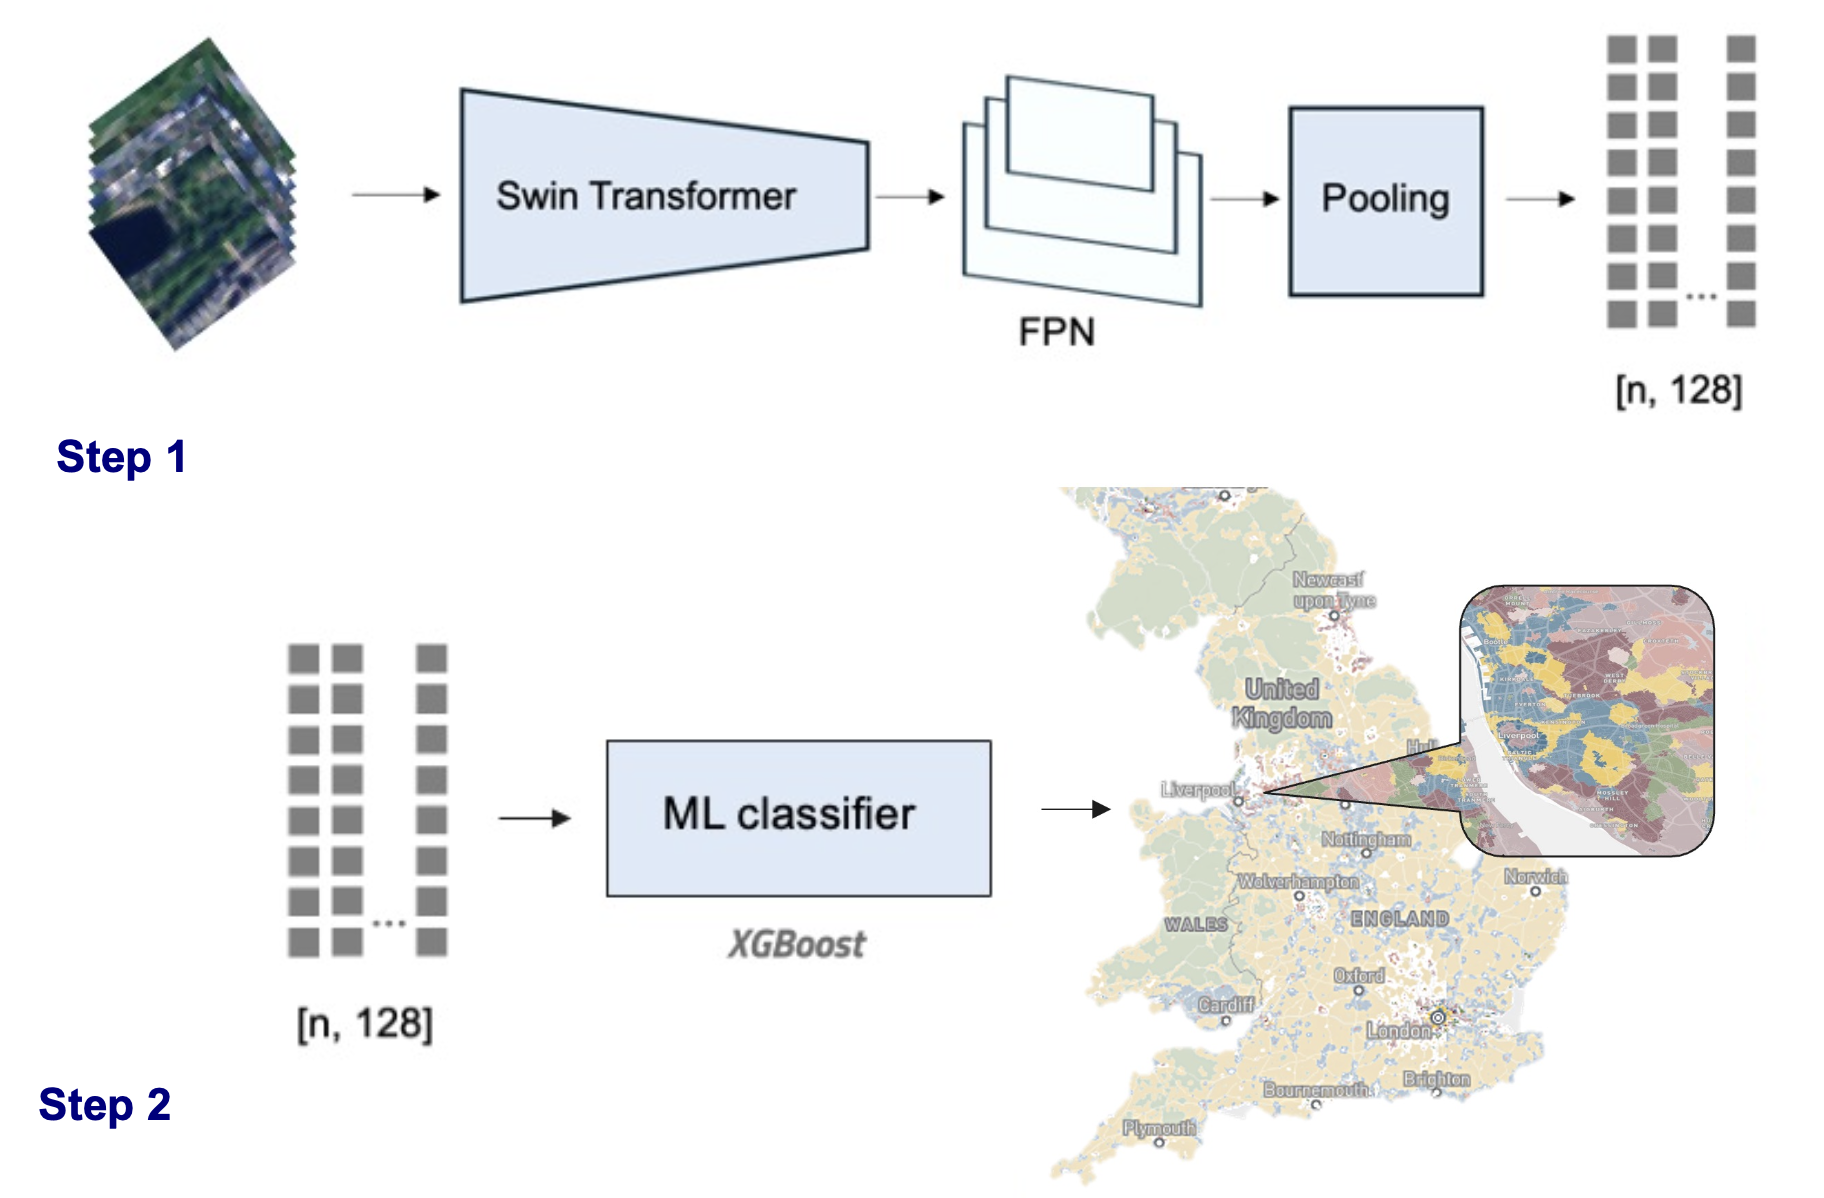
\includegraphics[width=\textwidth,height=4.16667in]{../figures/algo_design/baseline.png}
\end{center}

\begin{center}\rule{0.5\linewidth}{0.5pt}\end{center}

\subsection{Baseline: Results}\label{baseline-results}

\begin{center}
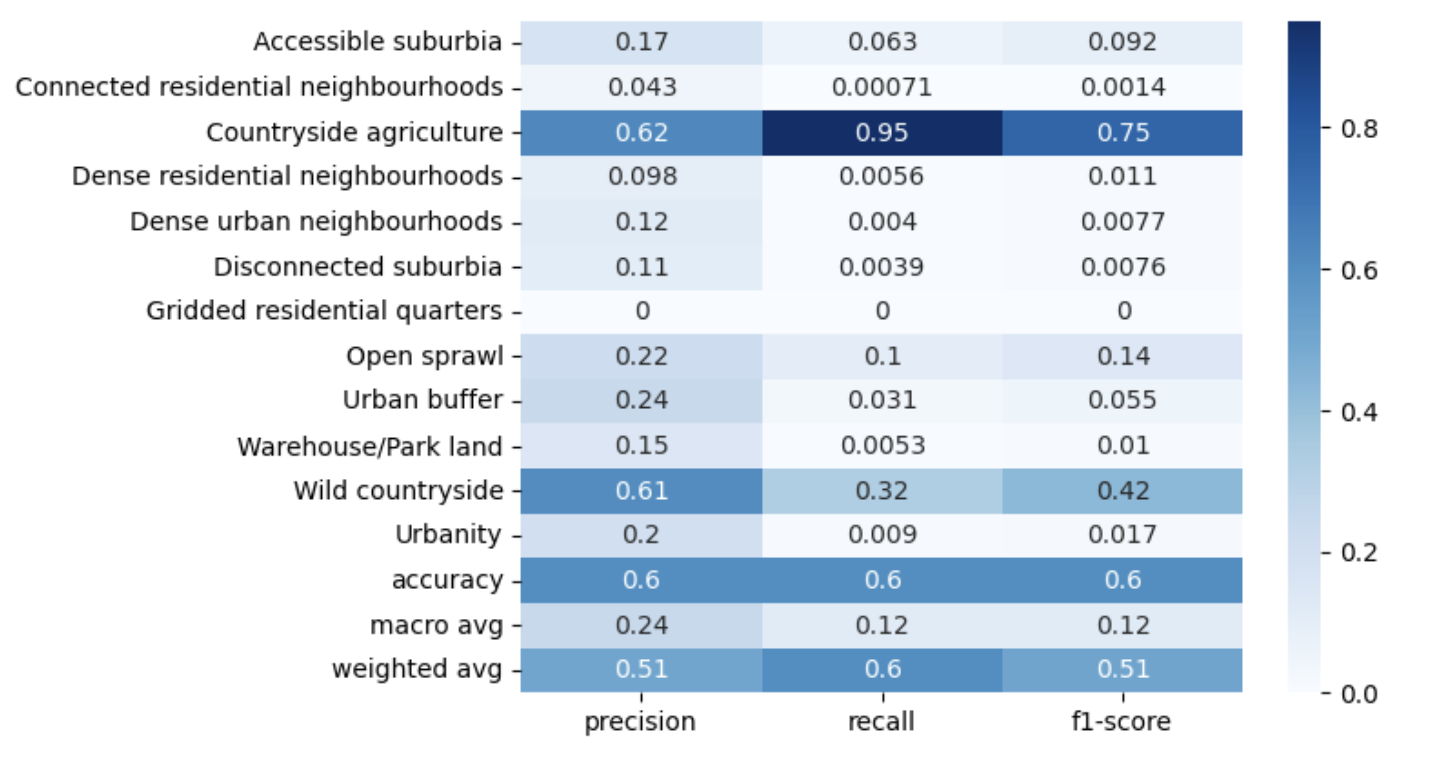
\includegraphics[width=\textwidth,height=4.375in]{../figures/algo_design/baseline_tile_level.png}
\end{center}

\section{WP 202: AI model design}\label{wp-202-ai-model-design}

\begin{center}
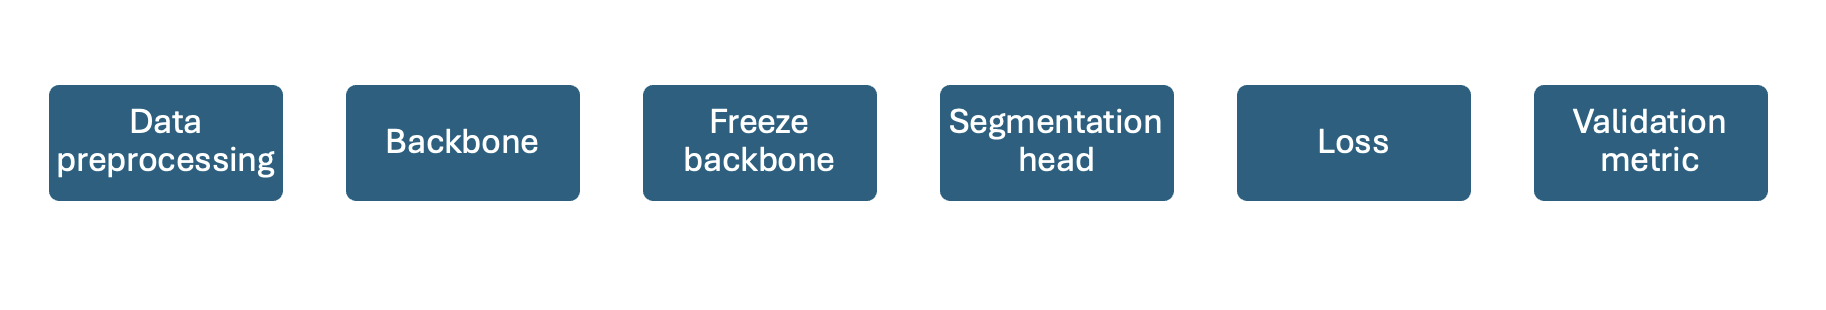
\includegraphics{../figures/algo_design/overview.png}
\end{center}

\subsection{Data preprocessing}\label{data-preprocessing}

\begin{itemize}
\tightlist
\item
  224 x 224 x 3 image tiles

  \begin{itemize}
  \tightlist
  \item
    26,942 tiles (.tif)
  \end{itemize}
\item
  Labels:

  \begin{itemize}
  \tightlist
  \item
    Spatial signatures (.tif)
  \end{itemize}
\item
  Train/test split: stratified 80/20\% (stratified by distribution in
  dataset)
\end{itemize}

\begin{center}\rule{0.5\linewidth}{0.5pt}\end{center}

\subsubsection{Train/test}\label{traintest}

80/20\% \begin{center}
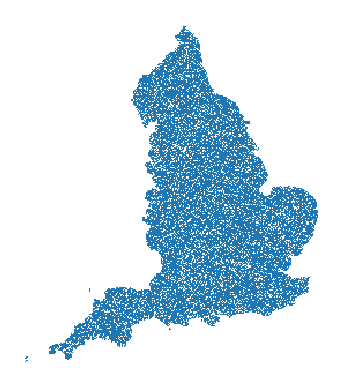
\includegraphics[width=\textwidth,height=4.16667in]{../figures/algo_design/train_df.png}
\end{center}
\begin{center}
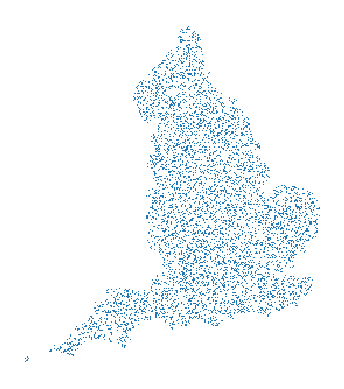
\includegraphics[width=\textwidth,height=4.16667in]{../figures/algo_design/test_df.png}
\end{center}

\begin{center}\rule{0.5\linewidth}{0.5pt}\end{center}

\subsubsection{Unbalanced dataset}\label{unbalanced-dataset}

\begin{center}
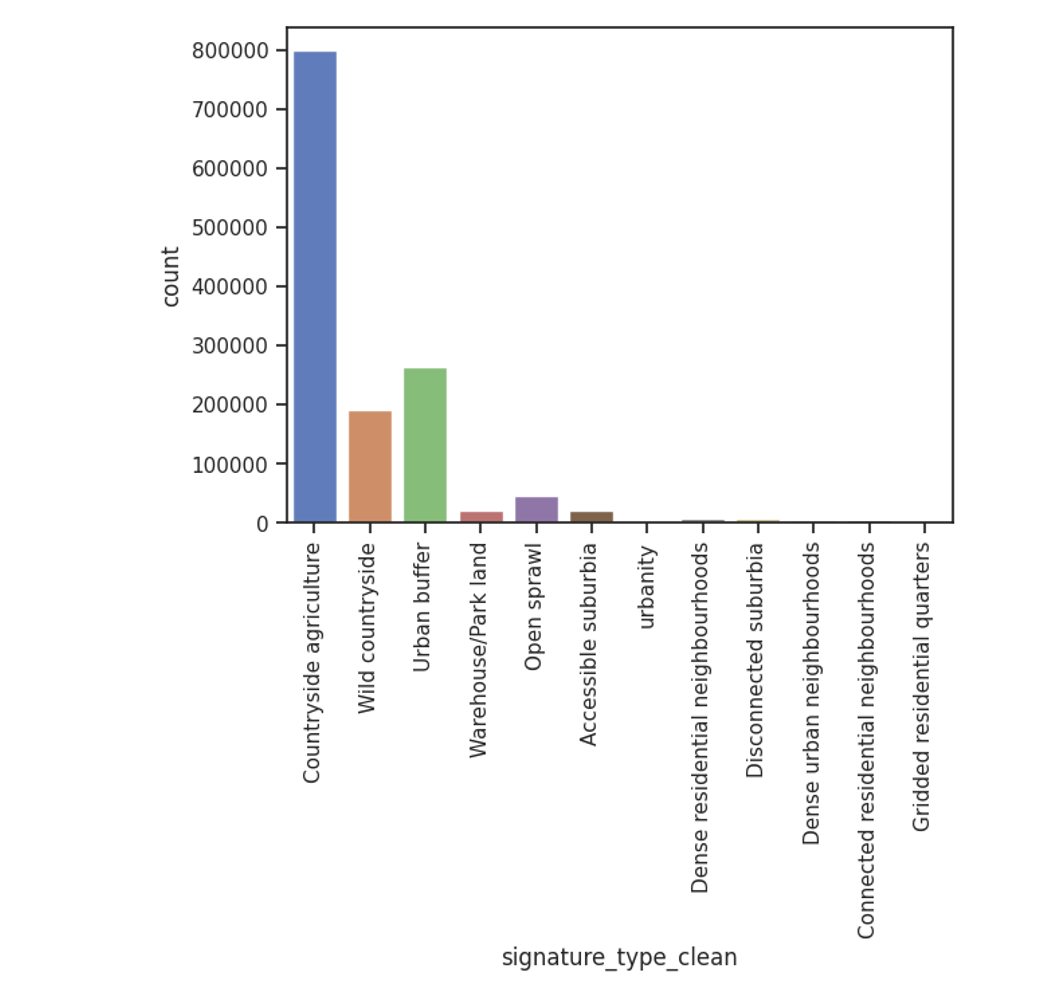
\includegraphics[width=\textwidth,height=4.375in]{../figures/algo_design/unbalanced.png}
\end{center}

\begin{center}\rule{0.5\linewidth}{0.5pt}\end{center}

\subsubsection{Example}\label{example}

\begin{center}
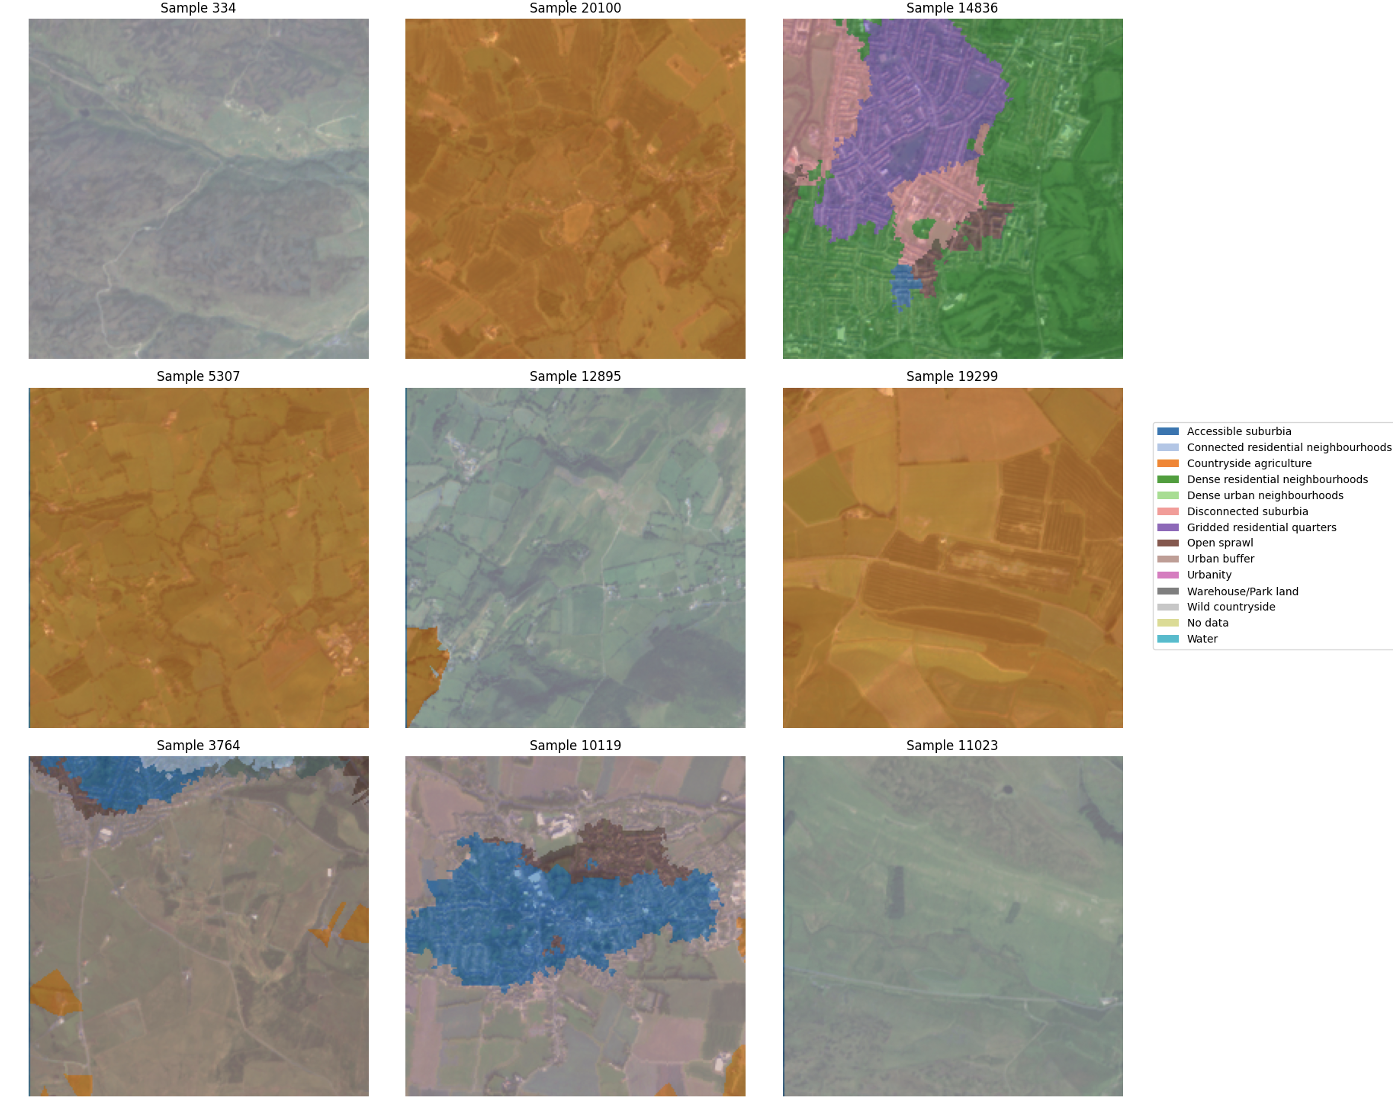
\includegraphics[width=\textwidth,height=4.375in]{../figures/algo_design/random_sample.png}
\end{center}

\begin{center}\rule{0.5\linewidth}{0.5pt}\end{center}

\subsection{Model design}\label{model-design}

\begin{center}
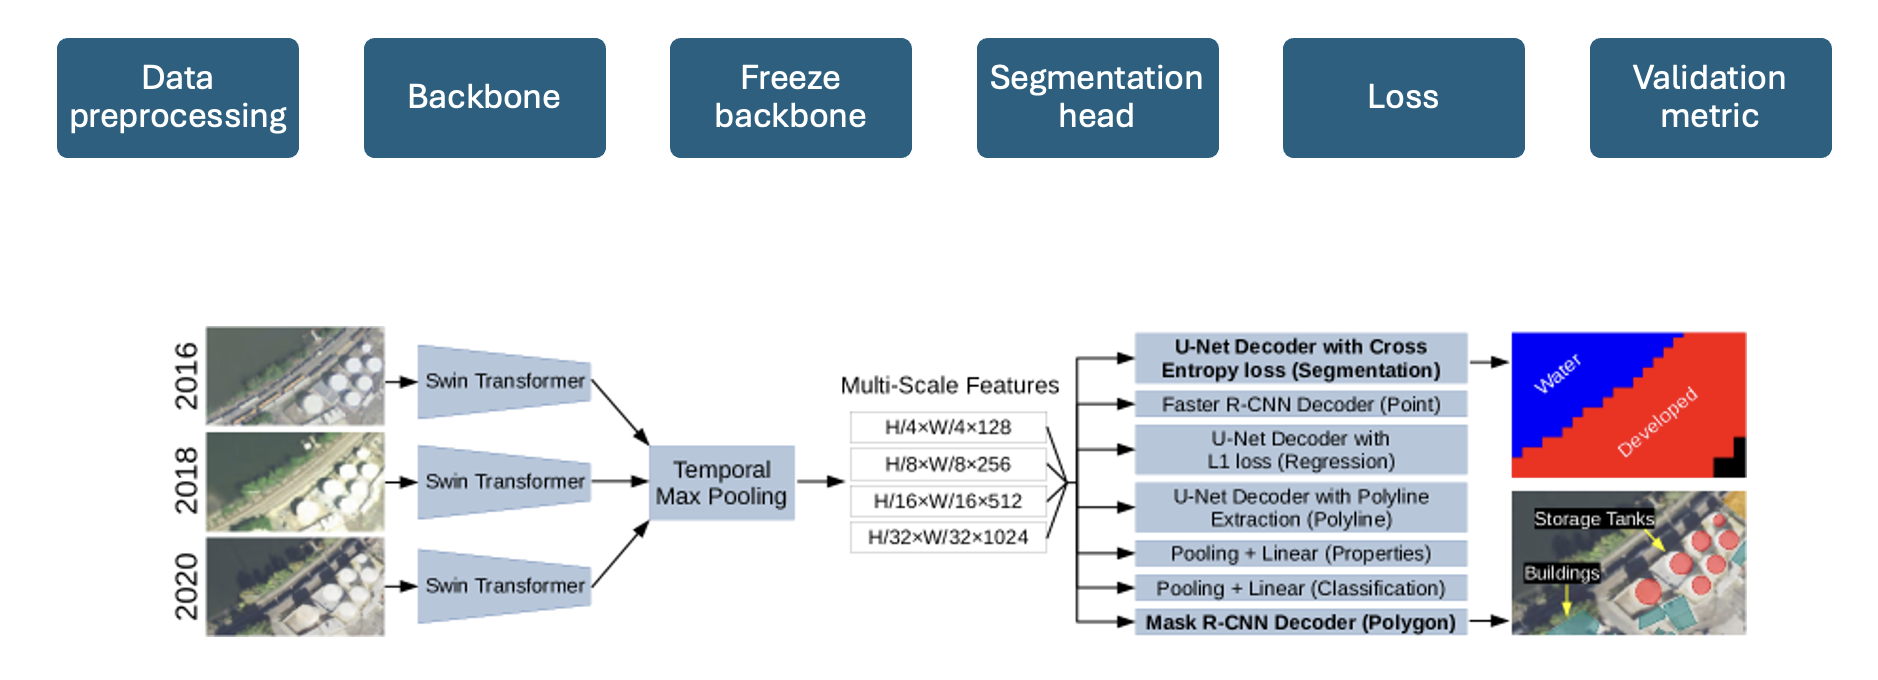
\includegraphics[width=\textwidth,height=4.16667in]{../figures/algo_design/example.png}
\end{center}

\subsection{Model design}\label{model-design-1}

\begin{center}
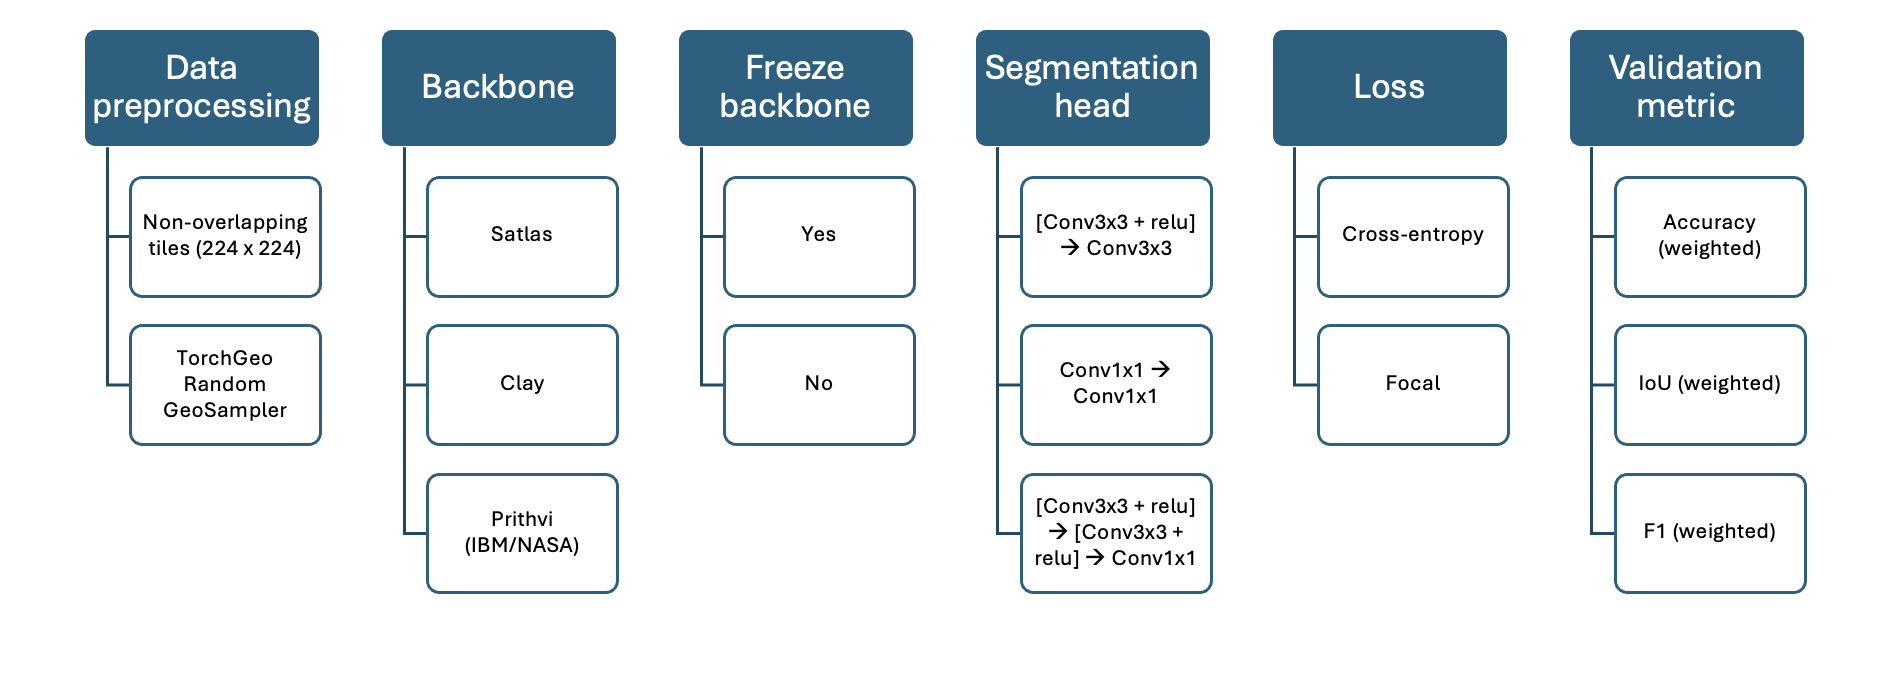
\includegraphics{../figures/algo_design/setup.png}
\end{center}

\subsection{Backbone: foundation
models}\label{backbone-foundation-models}

\begin{itemize}
\tightlist
\item
  Satlas
\item
  Clay
\item
  IBM/NASA (Prithvi)
\end{itemize}

\begin{center}
\includegraphics[width=\textwidth,height=2.08333in]{../figures/algo_design/foundation_models.png}
\end{center}

\begin{center}\rule{0.5\linewidth}{0.5pt}\end{center}

\subsection{Comparison of backbones}\label{comparison-of-backbones}

\begin{longtable}[]{@{}llrc@{}}
\toprule\noalign{}
Model & Architecture & \#Labels & Images \\
\midrule\noalign{}
\endhead
\bottomrule\noalign{}
\endlastfoot
Satlas & SwinT & 302M & Sentinel-2 \\
Clay & MAE/ViT & 70M & Sentinel-2/Landsat/NAIP/LINZ \\
Prithvi & MAE/ViT & 250 PB & Sentinel-2/Landsat \\
\end{longtable}

\subsection{Loss}\label{loss}

\begin{itemize}
\tightlist
\item
  \textbf{CrossEntropy Loss} (``ce''):

  \begin{itemize}
  \tightlist
  \item
    penalizes pixel-wise misclassifications
  \end{itemize}
\item
  \textbf{Focal Loss} (``focal''):

  \begin{itemize}
  \tightlist
  \item
    reduces the contribution of easily classified examples and puts more
    weight on hard-to-classify pixels.
  \end{itemize}
\end{itemize}

\subsection{Validation metric}\label{validation-metric}

\begin{itemize}
\tightlist
\item
  \textbf{IoU} (Intersection over Union)

  \begin{itemize}
  \tightlist
  \item
    Overlap between predicted and ground truth segmentations; 0 (no
    overlap) to 1 (perfect overlap).
  \end{itemize}
\item
  \textbf{F1 Score} (Weighted)

  \begin{itemize}
  \tightlist
  \item
    Balancing precision (how much of the prediction is correct) and
    recall (how much of the actual segmentation is captured).
  \end{itemize}
\item
  \textbf{Accuracy} (Weighted)

  \begin{itemize}
  \tightlist
  \item
    Percentage of correctly classified pixels.
  \end{itemize}
\end{itemize}

\begin{center}\rule{0.5\linewidth}{0.5pt}\end{center}

\subsubsection{Model A: Satlas}\label{model-a-satlas}

\begin{center}
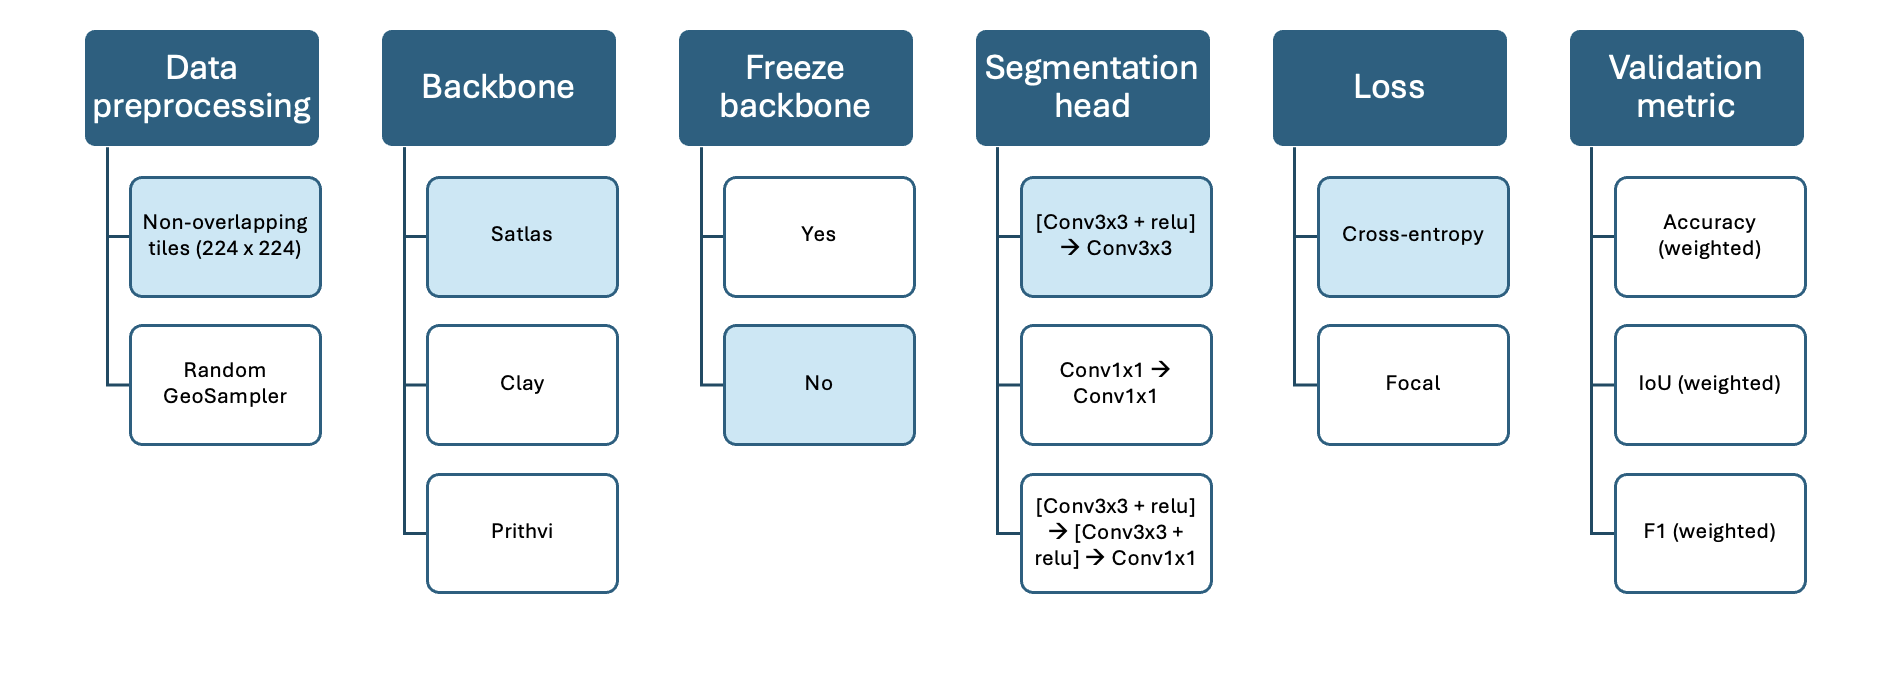
\includegraphics[width=\textwidth,height=4.16667in]{../figures/algo_design/satlas_model.png}
\end{center}

\begin{center}\rule{0.5\linewidth}{0.5pt}\end{center}

\subsubsection{Model B: Clay}\label{model-b-clay}

\begin{center}
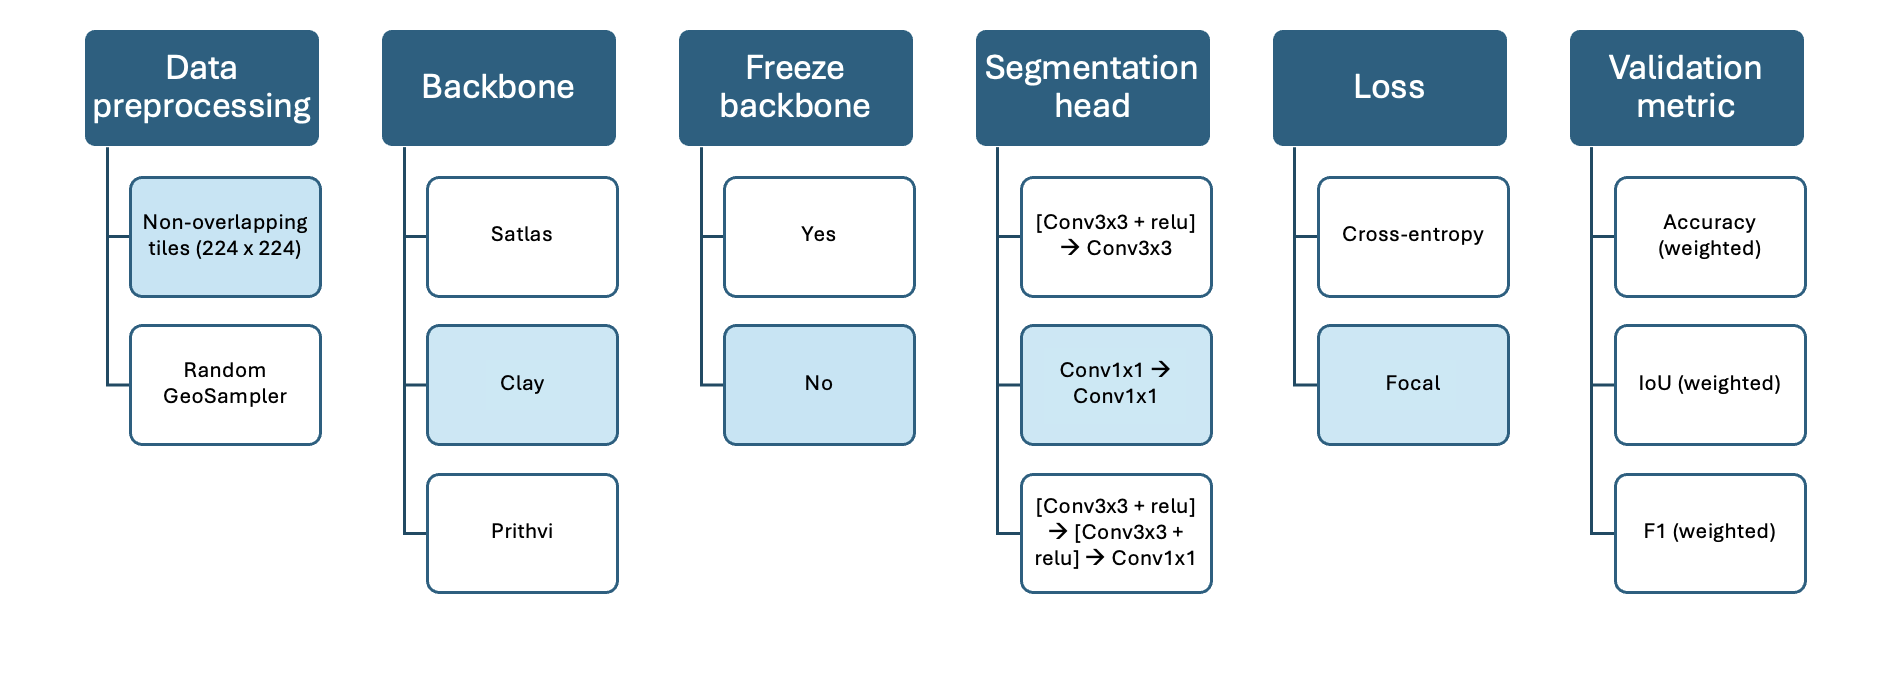
\includegraphics[width=\textwidth,height=4.16667in]{../figures/algo_design/clay_model.png}
\end{center}

\begin{center}\rule{0.5\linewidth}{0.5pt}\end{center}

\subsubsection{Model C: Prithvi}\label{model-c-prithvi}

\begin{center}
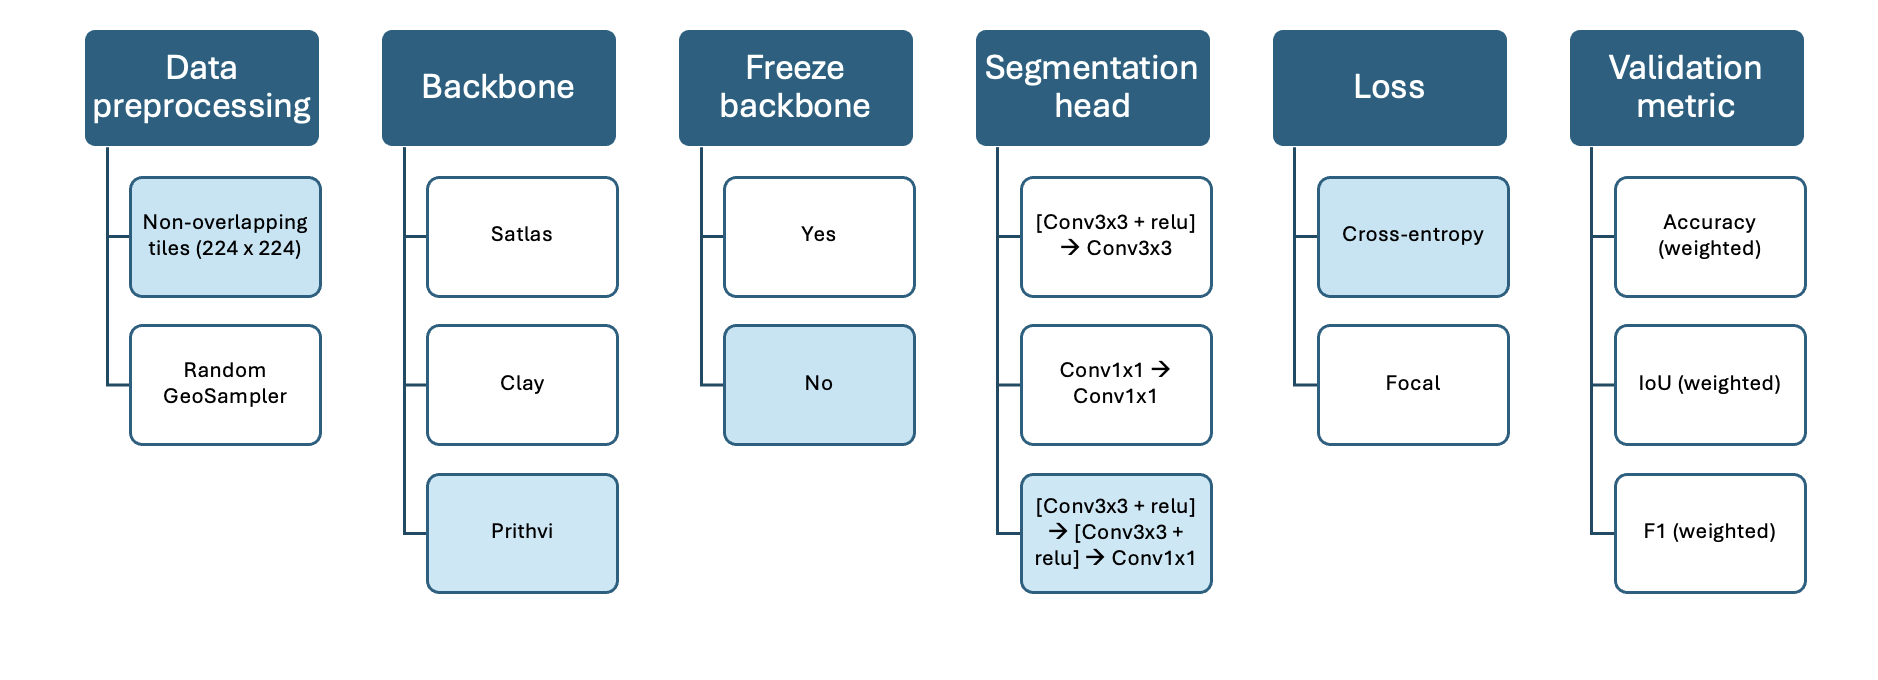
\includegraphics[width=\textwidth,height=4.16667in]{../figures/algo_design/prithvi_model.png}
\end{center}

\begin{center}\rule{0.5\linewidth}{0.5pt}\end{center}

\subsubsection{Results: fine-tuning}\label{results-fine-tuning}

\begin{longtable}[]{@{}llll@{}}
\toprule\noalign{}
Model & Satlas & Clay & Prithvi \\
\midrule\noalign{}
\endhead
\bottomrule\noalign{}
\endlastfoot
Run time (per epoch) (with GPU) & 9 mins & 8 mins & 20 mins \\
\# parameters & 90M & 86M & 120M \\
Implementation & 5/10 & 6/10 & 7/10 \\
Hyperparameter tracking & Own setup & Wandb.ai & Tensorboard \\
\end{longtable}

\begin{center}\rule{0.5\linewidth}{0.5pt}\end{center}

\subsubsection{Results: fine-tuning 10
epochs}\label{results-fine-tuning-10-epochs}

\begin{longtable}[]{@{}llll@{}}
\toprule\noalign{}
& Satlas & Clay & Prithvi \\
\midrule\noalign{}
\endhead
\bottomrule\noalign{}
\endlastfoot
Accuracy (weighted) & 0.57 & \textbf{0.72} & 0.62 \\
IoU (weighted) (0-1) & 0.33 & \textbf{0.58} & 0.41 \\
F1 (weighted) & 0.41 & \textbf{0.69} & 0.58 \\
\end{longtable}

Without hyperparameter tuning!

\begin{center}\rule{0.5\linewidth}{0.5pt}\end{center}

\subsubsection{Results: fine-tuning w/ focal
loss}\label{results-fine-tuning-w-focal-loss}

\begin{longtable}[]{@{}llll@{}}
\toprule\noalign{}
& Satlas & Clay & Prithvi \\
\midrule\noalign{}
\endhead
\bottomrule\noalign{}
\endlastfoot
Accuracy (weighted) & 0.25 & \textbf{0.72} & 0.59 \\
IoU (weighted) (0-1) & 0.2 & \textbf{0.58} & 0.42 \\
F1 (weighted) & 0.21 & \textbf{0.69} & 0.59 \\
\end{longtable}

\begin{center}\rule{0.5\linewidth}{0.5pt}\end{center}

\subsection{Prithvi: CE vs focal loss}\label{prithvi-ce-vs-focal-loss}

\begin{center}
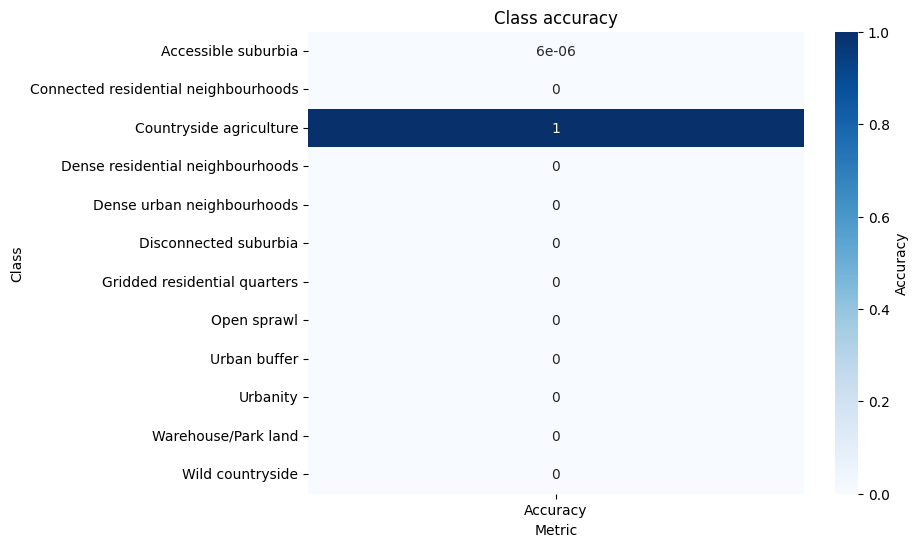
\includegraphics[width=\textwidth,height=3.125in]{../figures/algo_design/class_acc_ce_loss.png}
\end{center}
\begin{center}
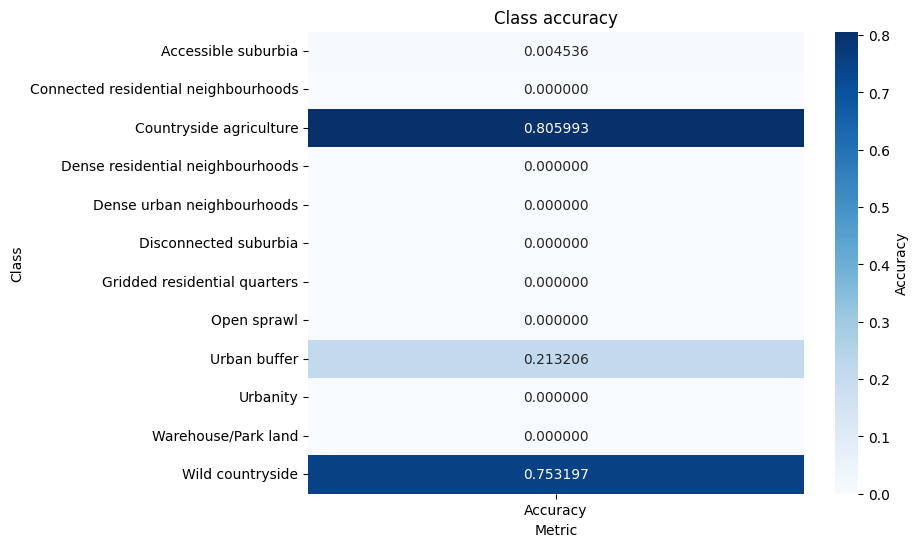
\includegraphics[width=\textwidth,height=3.125in]{../figures/algo_design/class_acc_focal_loss_prithvi.png}
\end{center}

\subsection{Clay predictions}\label{clay-predictions}

\begin{center}
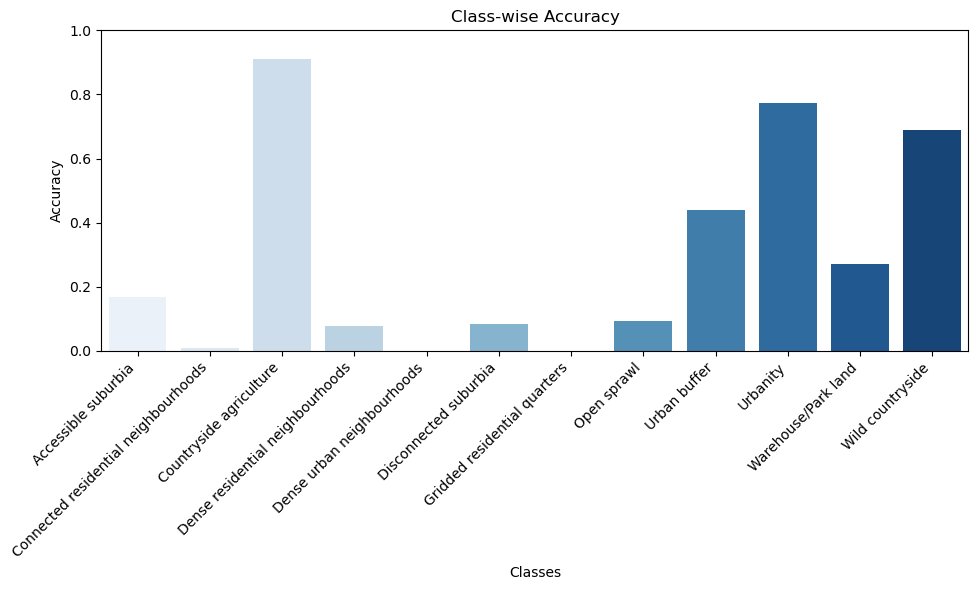
\includegraphics[width=\textwidth,height=4.47917in]{../figures/algo_design/class_acc.png}
\end{center}

\subsection{Summary: model comparison}\label{summary-model-comparison}

\begin{itemize}
\tightlist
\item
  Clay is the winner!
\item
  Training loss is important
\item
  Some classes still very much underdetected!
\end{itemize}

\#\#Main AI model We cut the UK satellite data into 26,942 image tiles
with shape 224 x 224 x 3 (RGB) The main model is based on a segmentation
task, in which we predict the spatial signatures on a pixel level. The
spatial signatures dataset is quite imbalanced. We carry out a
comparison between three foundation models as backbones: Satlas, Clay,
Prithvi. Based on our experiments, the model with Clay backbone
performed the best, and better than the baseline model with a weighted
accuracy of 0.72. The Clay model uses focal loss as loss function, which
could be the reason why the model performed better than the other models
that use cross entropy loss. We, thus, further implemented all models
with focal loss but the Clay model still performed best. Based on the
initial results, some classes are still very much underdetected and the
prediction performance is especially high for classes with lots of
training examples. For the next steps, we will look at hyperparameter
tuning for the Clay model and create a hierarchical approach, where we
first predict urban/non-urban classes and then in a second model predict
more detailed urban fabric. We are also working on finding good ways to
compare the classification with the segmentation model results (baseline
vs main AI model). This is a non-trivial task because the image tiles do
not correspond to each other and do not perfectly overlap (42px vs 224
px). The detailed results of the AI model development will be shared in
the technical note two weeks before the next progress meeting.



\end{document}
